\documentclass[aspectratio=169, bigger, xcolor={table}]{beamer}
\usepackage[magyar]{babel}
\usepackage{t1enc}
\usepackage{lipsum}
\usepackage{hulipsum}
\usepackage{mathtools}
\usepackage{colortbl}
\usepackage{amsthm}
\usepackage{enumerate}

\usetheme{CambridgeUS}
\usecolortheme{spruce}

\author{Görög Krisztina Erzsébet}
\title{Feladatok megoldása}
\subtitle{A feladat megoldás}
\institute{Miskolci Egyetem}
\date{\today}



\begin{document}
\maketitle
\AtBeginSection{\frame{\sectionpage}}
\AtBeginSection{\frame{%
\tableofcontents[sections={\value{section}}]}}

\section{Az első section}
\subsection{Valamik}

\begin{frame}{A frame címe}{Ez az alcím}
Ez itt ennek a frame-nek a tartalma.

A feladat szerint írni kell néhány sort.
\end{frame}

\begin{frame}[allowframebreaks]{Második frame}{2. alcím}
\hulipsum
\end{frame}

\begin{frame}{Harmadik frame}{Harmadik frame alcíme}
\begin{columns}[c]

\begin{column}{0.5\linewidth}
\begin{enumerate}
\item klsda
\item lksd
\item klasd
\item lksdf
\end{enumerate}

\begin{itemize}
\item kds
\item klsdjf
\item ksldkf
\end{itemize}
\end{column}

\begin{column}{0.5\linewidth}
\begin{figure}
\caption{Kép almákról}
\label{fig:almak}
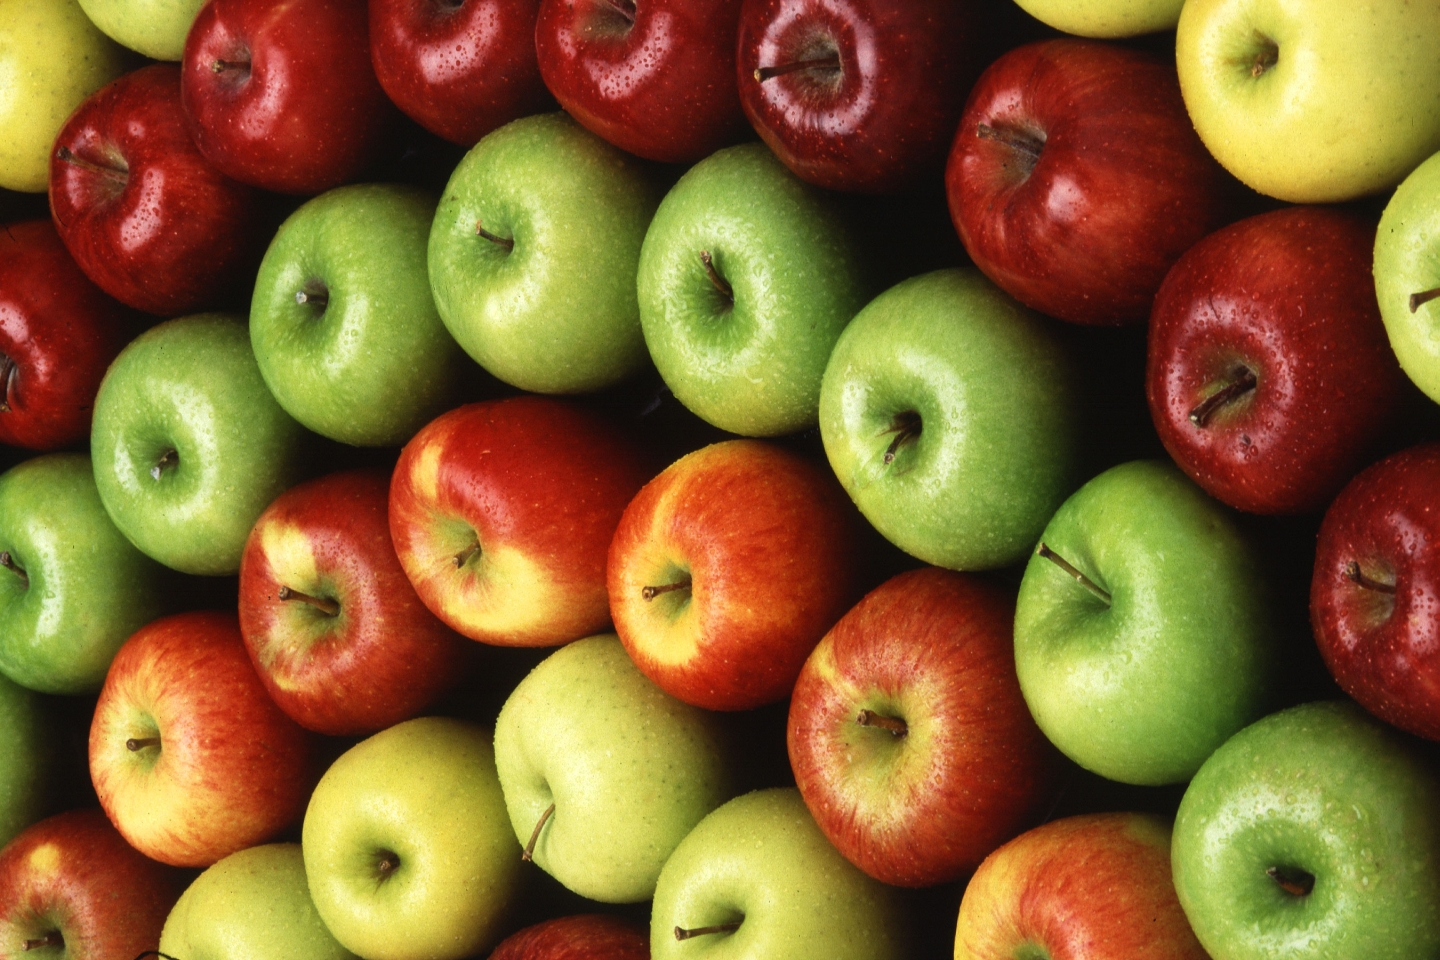
\includegraphics[height=5cm, width=5cm, keepaspectratio]{alma}

\end{figure}
\end{column}

\end{columns}
\end{frame}

\section{Második section}
\subsection{Még valami}
\begin{frame}{Negyedik frame}{Negyedik frame alcíme}
Ez itt ennek a frame-nek a tartalma.

A feladat szerint írni kell néhány sort.
\end{frame}

\begin{frame}[fragile]{Verbatimos frame}{Verbatim alcím}

\begin{verbatim}
\fjkd
slskjf
\ksdjfk
\ksdj
\end{verbatim}

\end{frame}

\subsection{Még több subsection}
\begin{frame}{Blokk tesztelés}{Blokkok}
\begin{block}{Blokk tesztelése}
block tartalma, ide valamit írni kéne
\end{block}

\begin{exampleblock}{Example}
exampleblock tartalma
\end{exampleblock}

\begin{alertblock}{Alertblokk tesztelés}
alertblock tartalma
\end{alertblock}

\end{frame}

\begin{frame}{Theorem, proof}{Ez az alcíme}
Ez itt ennek a frame-nek a tartalma.
\begin{theorem}[Ez egy theorem]
Ez a theorem szerint ez és ez...
\end{theorem}

\begin{proof}[Egy proof]
Ez itt pedig egy proof...
\end{proof}
\end{frame}

\begin{frame}{Semiverbatim}{Semiverbatimos dia}
\begin{semiverbatim}
\color{red}
\\begin\{enumerate\}

\\item valami

\\item valami

\color{blue}

\\begin\{enumerate\}

\\item még valami

\\item még vlammit

\\item jlsdk

\\end\{enumerate\}

\color{red}

\\item klsaj

\\end\{enumerate\}
\color{black}
\end{semiverbatim}
\end{frame}

\subsection{Még több!}
\begin{frame}{A frame címe}{Ez az alcím}
Ez itt ennek a frame-nek a tartalma.

A feladat szerint írni kell néhány sort.
\end{frame}

\begin{frame}{A frame címe}{Ez az alcím}
Ez itt ennek a frame-nek a tartalma.

A feladat szerint írni kell néhány sort.
\end{frame}

\end{document}